\chapter{System testing and test case design}
\section{Testing stages}
We interact with our systems through interfaces, such as CLIs and GUIs. These systems are in turn composed of subsystems which also has their own interfaces.\\
\\
System-level testing is about testing the whole system, or parts of it, through an interface. It integrates lower-level components. Many errors first occur when we try to connect several subsystems together, these are the main errors we are looking for in system-level testing.
\subsection{Unit vs System testing}
Unit is about testing a single class, implementation testing, while system testing is about testing the whole system, integration testing.\\
\\
Often we use the 70/20/10 model, 70\% unit testing, 20\% integration testing and 10\% UI testing. This is because without functioning units, of course the integration testing will fail, and without functioning integration between units, the UI testing will most likely fail.\\
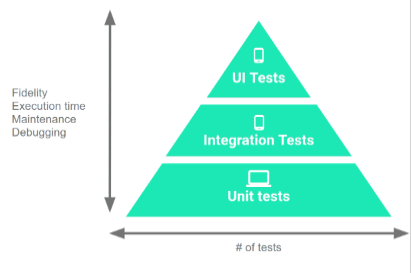
\includegraphics[width=0.5\pdfpagewidth]{lessons/images/70-20-10.png}\\

\section{Interface types}
\subsection{Parameter Interface}
Data passed through method parameters, the functions/methods you can call in a class.
\subsection{Procedural Interface}
An interface which surfaces a set of lower level functions to be able to be called by other components, an example of this is an API, or a GUI.
\subsection{Shared memory interface}
A block of memory shared between systems, a shared database, or data bus.
\subsection{Message-passing interface}
Instead of having two systems connected directly, an intermediary handles the sharing of messages between them.

\section{Interface errors}
\subsection{Interface misuse}
Malformed data, or a wrong number of parameters
\subsection{Interface misunderstanding}
Incorrect assumptions made about called component, e.g. binary search in unordered array.
\subsection{Timing errors}
The producer or consumer reads/writes in the wrong order.

\section{Creating System-level tests}

\begin{enumerate}
	\item Identify a function that can be tested in relative isolation.
	\item Identify controllable aspects of the input and environment that determine the outcome of the function.
	\item Identify types of values for each choice that lead to different function outcomes.
	\item Combine values to form "recipes" for test cases.
	\item Replace representative values with concrete values.
\end{enumerate}

Independently testable functionality are well defined functions, most often based on the "verbs". For UI-tests, look for functions visible to the user.

\section{Units and "Functionality"}
Many tests are written in terms of "units" of code. An independently testable function is a \textit{capability} of a unit.\\
\\
When testing functions we don't need to test every possible input, most inputs gets similar response, e.g. when testing a number input, maybe test negative, normal, zero, strings , and a large integer, not every single possible input.\\
\\
To figure out what to test, we usually divide all input into different partitions, and test from all partitions. Look att output events, ranges of values, membership groups, timing, and other aspects of the function.\\
\\
